
\section{Personal Histories}

The following sections will feature many of the same figures;
here we will introduce them so their interleaving stories may be told
uninterrupted in the following sections.
Readers unfamiliar with the history of Unix may find unfamiliar terms in these
personal accounts; these will be discussed in the following sections after
our characters have been introduced.

\subsection{Doug McIlroy, Joined 1958}

Douglas McIlroy joined Bell Labs in 1958 and shortly thereafter earned his
PhD in applied mathematics from MIT.
McIlroy became head of the Computing Techniques Research department in 1965, and he's regarded
as one of the most brilliant members of the staff by key members that readers may be more familiar with.

He is described by nearly everyone at the Bell Labs Computing Research Center
(who wrote or spoke about their time there)
as the most brilliant member of that team that no one has heard of
\cite{kernighan_interviews_thompson_2019}; Ken Thompson described him as
"the smartest one of all of us and the least remembered or written down of all of us."

He was relatively hands-off as a manager, preferring to peek into his employees' offices
with suggestions or interesting problems and wait for the employees to let \textit{him} know
what needed to be done, rather than assigning tasks directly.
His employees respected his tasted in technical and personal matters,
as Brian Kernighan describes\cite{kernighan_unix:_2020}:

\begin{quotation}
Unix might not have existed, and certainly
would not have been as successful, without Doug's good taste and sound
judgment of both technical matters and people.
\end{quotation}

\begin{figure}
    \centering
    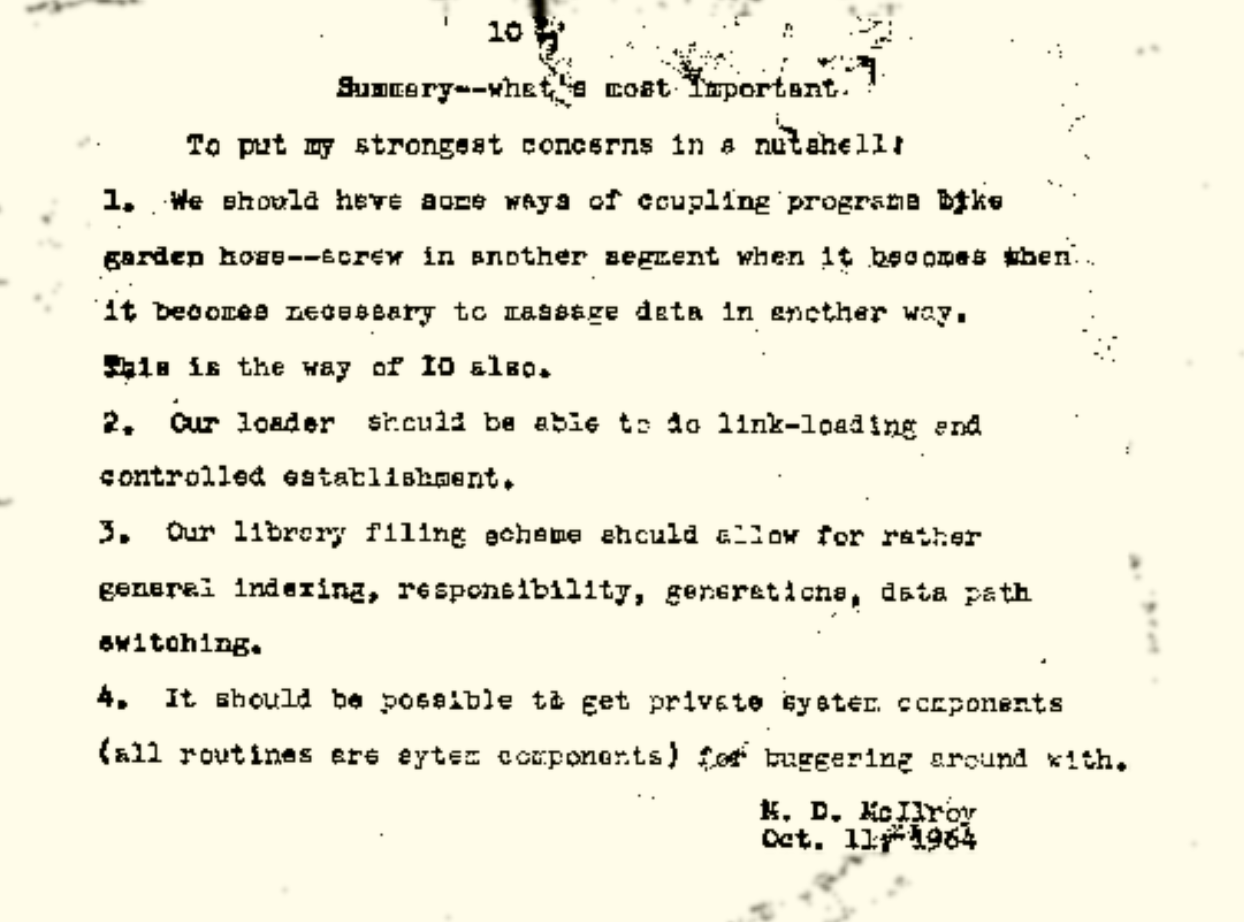
\includegraphics[width=0.7\textwidth]{resource/software/unix/doug-1964-pipes.png}
    \caption{Doug McIlroy's 1964 memo proposing Unix pipes\cite{doug_mcilroy_origin_of_unix_pipes_1964}.}
    \label{fig:unix-pipes-mcilroy-memo}
\end{figure}

In 1964, he circulated a memo which led to Unix pipes\cite{doug_mcilroy_origin_of_unix_pipes_1964}
(see \ref{fig:unix-pipes-mcilroy-memo}) though it took him quite a while to convince
Ken Thompson that he really ought to implement them.

He hired Alfred Aho in 1967\cite{aho_oral_history_2022}:

\begin{quotation}
I was interviewed by a department head by the name of Doug McIlroy. He was an applied
mathematician from MIT. He had been at Bell Labs for a few years before me. Amongst other things, he
had co-invented macros for programming languages and he's also in this class of one of the smartest
people I've ever met.
\end{quotation}

\subsection{Ken Thompson, Joined 1966}



\subsection{Dennis Ritchie, Joined 1967}



\subsection{Alfred Aho, Joined 1967}



\subsection{Jeffrey Ullman, Joined 1967}



\subsection{Brian Kernighan, Joined 1969}
